\documentclass[conference]{IEEEtran}
\IEEEoverridecommandlockouts
% The preceding line is only needed to identify funding in the first footnote. If that is unneeded, please comment it out.
\usepackage{cite}
\usepackage{amsmath,amssymb,amsfonts}
\usepackage{algorithmic}
\usepackage{graphicx}
\usepackage{textcomp}
\usepackage{xcolor}
\usepackage{listings}
\def\BibTeX{{\rm B\kern-.05em{\sc i\kern-.025em b}\kern-.08em
    T\kern-.1667em\lower.7ex\hbox{E}\kern-.125emX}}
\begin{document}

\title{RFID Sicherheit}


\author{\IEEEauthorblockN{Julian Hoever}
\IEEEauthorblockA{\textit{Verteilte Systeme} \\
\textit{Universität Duisburg-Essen}\\
Duisburg, Deutschland\\
julian.hoever@stud.uni-due.de}
}

\maketitle

\begin{abstract}
Die folgende Arbeit behandelt das Thema der RFID Sicherheit im Bezug auf Sicherheitslücken, Schutzmaßnahmen und Privatsphäre. Es werden einige mögliche Schwachstellen der RFID/NFC Technik aufgezeigt und Angriffstechniken vorgestellt, welche die zuvor aufgeführten Schwachstellen ausnutzen. Dabei wird darauf eingegangen, in welchen realen Szenarien diese Angriffe eine Bedrohung darstellen, wie zum Beispiel beim kontaktlosen Bezahlen oder der Diebstahlsicherung von Waren. Anschließend werden einige Schutzmaßnahmen skizziert, welche die zuvor genannten Angriffstechniken abmildern oder verhindern können und es wird diskutiert, wie durchführbar die genannten Angriffstechniken in der realen Welt sind. Dies hilft dabei abzuschätzen, wie relevant die Bedrohung ist, die von der RFID Technik in diesen Bereichen ausgeht. Abschließend wird noch der Aspekt der Einschränkung der Privatsphäre durch RFID Chips, besonders in Ausweisen aber auch in Produkten zur Diebstahlsicherung, besprochen und eingeordnet.
\end{abstract}

\section{Einleitung}
Die kontaktlose RFID Technik gehört bei vielen Menschen mittlerweile zum Alltag. Man nutzt sie um kontaktlos seinen Einkauf zu bezahlen, auf der Arbeit mittels RFID Transponders die Eingangstür zu öffnen und bei einer Stempeluhr seine Arbeitszeit zu dokumentieren. Die Einsatzbereiche der RFID Technik sind mittlerweile vielfältig. Eine weitere häufige Anwendung ist das Identifizieren von Gegenständen, zum Beispiel bei der Diebstahlsicherung von Waren oder der Verfolgung von Frachten. Durch die kontaktlosen Anwendungsbereiche bietet diese Technik einen erhöhten Komfort. Dafür zahlt man in vielen Fällen aber den Preis eines signifikant verringerten Sicherheitsniveaus oder eine Einschränkung der Privatsphäre. Um eine Einschränkung der Sicherheit und Privatsphäre zu verhindern, müssen durch geeignete Schutzmaßnahmen Systeme die auf RFID beruhen abgesichert werden und dabei auch, falls erforderlich, Maßnahmen zu Schutz der Privatsphäre getroffen werden.

Aus diesem Grund wird in dieser Arbeit dargestellt, was die Probleme und möglichen Angriffsszenarien der RFID/NFC Technik sind. Dabei werden ausschließlich die passive RFID Transponder behandelt, da diese durch den einfachen Aufbau und das Fehlen einer eigenen Stromversorgung sehr weit verbreitet sind.

Zu Beginn wird dazu in Abschnitt 2 auf die Grundlagen der RFID/NFC Technik eingegangen. Anschließend beschreibt Abschnitt 3 was RFID/NFC konzeptionell für Schwachstellen besitzt. Darauf aufbauend wird dann in Abschnitt 4 erläutert was sich für mögliche Angriffe, auf die Sicherheit des Systems und die Privatsphäre der Nutzer, aus den in Abschnitt 3 genannten Schwachstellen ergeben. In Abschnitt 5 werden mögliche Sicherheitsmaßnahmen skizziert, welche Angriffe auf diese Technik erschweren und in Abschnitt 6 wird diskutiert wie durchführbar die vorgestellten Angriffe auf RFID Systeme in der Praxis überhaupt sind.


\section{Grundlagen}

\subsection{RFID Technik}
Radio Frequency Identification (RFID) ist eine Technik um kontaktlos Daten mittels eines Lesegerätes (Transceiver) aus einem Transponder auszulesen. Transponder gibt es in vielen verschiedenen Formen und Größen, je nach Anwendungsbereich. Grundlegend funktionieren alle Transponder aber recht ähnlich. Transponder bestehen in der Regel aus einer Antenne, in Form einer Spule, Schaltkreisen zum Senden/Empfangen und einem Speicher. Die Kommunikation erfolgt dann wie in Fig. \ref{fig1} dargestellt.

\begin{figure}[htbp]
\centerline{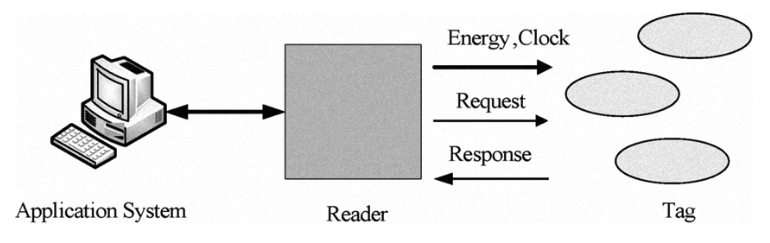
\includegraphics[width=0.5\textwidth]{img/kommunikation.png}}
\caption{Kommunikation zwischen Lesegerät (Reader) und Transponder \cite{b1}}
\label{fig1}
\end{figure}

Das Lesegerät (Reader) induziert über die spulenförmig angeordnete Antenne des Transponders, eine Spannung und Taktfrequenz, welche den Transponder mit dem nötigen Strom versorgt damit eine Kommunikation zwischen Lesegerät und Transponder stattfinden kann. Anschließend sendet das Lesegerät eine Anfrage an den Transponder, woraufhin ihm der Transponder seine Daten die er enthält übermittelt.

Bei den RFID Transpondern wird unterschieden zwischen passiven und aktiven Transpondern.
\begin{itemize}
\item Passive Transponder besitzen keine eigene Spannungsquelle und erreichen dadurch lediglich eine Reichweite von weniger als 4 Metern \cite{b1}.
\item Aktive Transponder hingegen besitzen zusätzlich noch eine eingebaute Spannungsquelle, meist in Form einer Batterie. Dadurch sind Reichweiten von über 100 Metern möglich \cite{b1}.
\end{itemize}
Wie bereits in der Einleitung angemerkt fokussiert sich diese Arbeit ausschließlich auf die passiven Transponder, da diese in im alltäglichen Leben, im Gegensatz zu den aktiven Transpondern, von größerer Bedeutung sind.

\subsection{NFC Technik}
NFC steht für Near Field Communication und ist ein Standard der der mit einer Frequenz von 13.56 MHz und einer Übertragungsgeschwindigkeit von 424 KBit/s arbeitet \cite{b2}. Dieser Standard ist für Datenübertragungen von bis zu 10 cm ausgelegt und setzt technisch direkt auf der RFID Technik auf \cite{b2}. Dies ermöglicht mittels eines NFC Lesegeräts, beispielsweise Smartphones, sogar RFID Transponder auszulesen. Zum Lesen und Schreiben wird auch hier ebenfalls mit einer spulenförmigen Antenne gearbeitet.

NFC kann in 3 Betriebsmodi betrieben werden \cite{b2}:

\begin{itemize}
\item Peer-to-Peer Modus
\item Lese-Schreib Modus
\item Kartenemulationsmodus
\end{itemize}

Bei dem Peer-to-Peer Modus findet zwischen beiden Geräten ein bidirektionaler Datenaustausch statt. Ein Beispiel dafür ist der Datenaustausch zwischen zwei Smartphones per NFC. Dabei agieren beide Smartphones als Sender und Empfänger.

Bei dem Lese-Schreib Modus fungiert das aktive Gerät als Lesegerät und das passive Gerät ist hierbei ein kompatibler passiver RFID Transponder zum Beispiel in einem Aufkleber oder einer Karte mit eingebautem RFID Transponder. Es ist in diesem Modus aber auch möglich, dass das aktive Gerät einen RFID Transponder, welcher noch nie beschrieben wurde, beschreibt.

Bei dem Kartenemulationsmodus simuliert das NFC Gerät einen passiven RFID Transponder was bedeutet, das dieses Gerät keinerlei Berechnungen durchführt und lediglich die festgelegten Daten an ein anfragendes Lesegerät übermittelt. Dies findet zum Beispiel beim kontaktlosen Bezahlen mittels Smartphone Anwendung.


\section{Schwachstellen}
Die RFID und NFC Technik besitzt vielerlei Schwachstellen und diese sind zum Großteil sowohl auf RFID als auch auf NFC anzuwenden. Der wichtigste Unterschied zwischen RFID und NFC ist die Reichweite auf denen diese Technik operiert. Bei NFC muss der Angriff viel näher am Lesegerät stattfinden als bei RFID, da mit passiven RFID Transpondern Reichweiten von bis zu 4 Metern erreicht werden können. Im folgenden werden einige mögliche Schwachstellen beider Techniken aufgelistet.

\subsection{Authentifikation}
Wie bereits in dem Abschnitt mit den Grundlagen der RFID Technik beschrieben, übermittelt ein RFID Transponder im wesentlichen seinen gesamten Speicherinhalt an ein anfragendes Lesegerät. Das bedeutet, dass keinerlei Authentifikation auf Seiten des Transponders stattfindet und damit jedes Lesegerät was auf der Frequenz des Transponders agiert den Transponder lesen kann, wodurch möglicherweise Daten in falsche Hände gelangen können. Jedoch gibt es seit einiger Zeit Transponder, welche eine Authentifikation durchführen bevor Daten übermittelt werden.

\subsection{Lesegerät kennt Daten nicht}
Ein weiteres Problem ist, dass das Lesegerät, welches Daten von einem Transponder anfragt, nicht weiß was für Daten es von dem Transponder erhält. Diese Daten müssen aber trotzdem verarbeitet werden, was ohne Sicherheitsvorkehrungen dazu führen kann, dass verarbeitende Prozesse oder Datenbanken, welche diese Daten speichern sollen, Schaden nehmen können.

\subsection{Eindeutige Identifikation}
Des Weiteren lässt sich sowohl der Speicherinhalt als auch die eindeutige Identifikationsnummer des Transponders dazu verwenden diesen zu identifizieren. Dies ist in vielen Situationen vermutlich gewünscht, kann aber auch ein Sicherheitsrisiko darstellen.

\subsection{Energieversorgung}
Damit ein passiver RFID Transponder funktionieren kann muss durch das Lesegerät eine Spannung induziert werden, welche dafür sorgt, dass der Transponder Daten versenden kann. Wird der RFID Transponder zum Beispiel durch einen Faradayschen Käfig abgeschirmt, wird der RFID Transponder nicht mit Energie versorgt und das Lesegerät bekommt keine Daten von dem RFID Transponder übermittelt.

\subsection{Übertragung}
Ursprünglich ist RFID mit dem Standard ISO/IEC 18000 so standardisiert worden, dass die Übertragung zwischen Lesegerät und Transponder im Klartext geschieht. Dies sorgt dafür, dass die Übertragung abgehört werden kann.

\section{Angriffe auf Sicherheit und Privatsphäre}
Mit den im vorherigem Abschnitt beschriebenen Schwachstellen lassen sich mögliche Angriffsszenarien beschreiben welche die Sicherheit eines Systems ohne entsprechende Gegenmaßnahmen gefährden würden.

\subsection{Kopieren von Transpondern}
Bei der Verwendung von Transpondern ohne Authentifikation lässt sich der Transponder ohne weiteres mit einem kompatiblen Lesegerät auslesen. Die ausgelesenen Daten können anschließend dazu verwendet werden einen neuen uninitialisierten Transponder zu beschreiben um dadurch eine Kopie des ursprünglich gelesenen Transponders zu erhalten. Diese Kopie kann dann den gleichen Zweck erfüllen wie das Original. Angenommen der Originaltransponder wurde dazu verwendet eine Haustüre zu öffnen. Das bedeutet, dass man durch ein kurzes Auslesen des Originaltransponders dazu in der Lage ist einen zweiten Hausschlüssel zu erzeugen.

\subsection{Kom­pro­mit­tie­ren des Lesegerätes}
Die Möglichkeit einfach einen RFID/NFC Transponder auszulesen stellt nicht nur ein Problem für die Sicherheit der Daten auf dem Transponder da. Durch das einfache Auslesen kann auch die Sicherheit des Lesegerätes und der darunter liegenden Softwareinfrastruktur entstehen. Dieses Problem entsteht dadurch, dass ein Lesegerät jeden Transponder liest, welcher sich in Reichweite ist. Befindet sich unter diesen Transpondern ein Transponder welcher Schadcode als Daten enthält, wird das Lesegerät, beispielsweise ein Smartphone oder eine Türsteuerung, dessen Daten ebenfalls lesen und verarbeiten. Wird auf Seiten des Lesegerätes nun nicht dafür gesorgt, dass Schadcode unschädlich gemacht wird, kommt dieser Schadcode ungehindert in tiefere Systembereiche.
Durch die verhältnismäßig kleine Speichergröße eines RFID Transponders von Bytes bis wenigen Kilobytes, beispielsweise 4 kB bei der MIFARE Classic EV1 4K \cite{b3}, ist die Größe des Schadcodes begrenzt, reicht aber aus um Schaden anzurichten \cite{b4}. Bei dem Schadcode kann es sich beispielsweise um SQL Injections handeln. Ein Beispielszenario wäre, dass ein Transponder mit einem schädlichen SQL Statement wie
\begin{lstlisting}
"; DROP TABLE <tabellenname>
\end{lstlisting}
\cite{b4} präpariert worden ist und dieser dann in die Nähe eines Lesegerätes gebracht wird. Das Lesegerät würde dann die Daten lesen und möglicherweise versuchen diese Daten in eine Datenbank zu schreiben. Das würde in der Datenbank dafür sorgen, dass die Tabelle mit dem in der SQL Injection angegebenen Tabellennamen gelöscht wird. Durch den Datenverlust entstehen in der Regel schwere Schäden auf Seiten des Lesegerätes und der dahinterstehen Softwareinfrastruktur.

\subsection{Erweitern von NFC zu Bluetooth}
Ein ähnliches Problem, was aber speziell NFC betrifft, ist die Koppelung von Bluetooth Verbindungen mittels NFC oder das Teilen von größeren Datenmengen eingeleitet über NFC. Dieses Angriffsszenario betrifft hauptsächlich Smartphones. Smartphones mit NFC besitzen oft die Möglichkeit über NFC Bluetooth Verbindungen herzustellen oder Daten zu teilen indem man lediglich das Smartphone in die Nähe des anderen Gerätes bringt. Beim Teilen von größeren Datenmengen über NFC wird auch häufig NFC nur zum Koppeln einer Bluetooth Verbindung genutzt und der eigentliche Datentransfer läuft anschließend über diese Bluetooth Verbindung \cite{b5}. Das Problem dabei ist, dass so die Kurzstreckenverbindung über NFC erweitert wurde auf eine Bluetooth Verbindung mit einer deutlich erhöhten Reichweite und einer schnelleren Übertragungsrate \cite{b5}. Diese Verbindung kann anschließend dafür genutzt werden aus größerer Entfernung Schadcode auf das Zielgerät zu schleusen.

\subsection{Tracking durch Transponder IDs}
Ein weiteres Problem ist die eindeutige Identifikationsnummer eines RFID Gerätes. Jedes RFID Gerät besitzt eine eindeutige Identifikationsnummer welche benötigt wird um Kollisionen bei der Übertragung zu verhindern \cite{b6}. Diese Identifikationsnummer bestimmt jeden Transponder und jedes RFID Gerät (und damit auch NFC Gerät) eindeutig und ermöglicht damit ein Tracking dieser Geräte. Dadurch kann massiv die Privatsphäre von Personen beeinträchtigt werden. Ein Szenario in dem diese Technik ausgenutzt werden könnte ist beispielsweise ein Unternehmen, in dem jeder Mitarbeiter RFID Transponder zum Zeitstempeln an Stempeluhren, Bezahlen in der Mensa und/oder zur Zugangskontrolle besitzt. Das Unternehmen könnte in dem Betrieb an vielen verschiedenen Stellen RFID Lesegeräte installieren. Diese Lesegeräte würden die Identifikationsnummer jedes RFID Transponders lesen, welcher in seine Reichweite kommt. Die Identifikationsnummer lassen sich dann Mitarbeitern zuordnen. Dadurch ist es möglich unbemerkt sämtliche Bewegungen der Mitarbeiter im Gebäude zu verfolgen. Diese Bewegungsprofile könnten anschließend dazu genutzt werden deren Arbeitszeit zu überwachen oder personelle Entscheidungen zu treffen.


\section{Sicherheitsmaßnahmen}
[WORK IN PROGRESS]


\section{Durchführbarkeit der Angriffe}
[WORK IN PROGRESS]


\section{Fazit}
[WORK IN PROGRESS]


\begin{thebibliography}{00}
\bibitem{b1} Chih-Yung Chen, Chien-Ping Kuo and Fang-Yuan Chien, "An exploration of RFID information security and privacy," 2009 Joint Conferences on Pervasive Computing (JCPC), Tamsui, Taipei, 2009, pp. 65-70, doi: 10.1109/JCPC.2009.5420211.

\bibitem{b2} N. A. Chattha, "NFC — Vulnerabilities and defense," 2014 Conference on Information Assurance and Cyber Security (CIACS), Rawalpindi, 2014, pp. 35-38, doi: 10.1109/CIACS.2014.6861328.

\bibitem{b3} NPX Semiconductors (32, November 2017) MIFARE Classic EV1 4K - Mainstream contactless smart card IC for fast and easy solution development. [Online]. Available: https://www.nxp.com/docs/en/data-sheet/MF1S70YYX\_V1.pdf.

\bibitem{b4} M. R. Rieback, B. Crispo and A. S. Tanenbaum, "Is your cat infected with a computer virus?," Fourth Annual IEEE International Conference on Pervasive Computing and Communications (PERCOM'06), Pisa, 2006, pp. 10 pp.-179, doi: 10.1109/PERCOM.2006.32.

\bibitem{b5} R. Verdult and F. Kooman, "Practical Attacks on NFC Enabled Cell Phones," 2011 Third International Workshop on Near Field Communication, Hagenberg, 2011, pp. 77-82, doi: 10.1109/NFC.2011.16.

\bibitem{b6} G. Madlmayr, J. Langer, C. Kantner and J. Scharinger, "NFC Devices: Security and Privacy," 2008 Third International Conference on Availability, Reliability and Security, Barcelona, 2008, pp. 642-647, doi: 10.1109/ARES.2008.105.
\end{thebibliography}
\end{document}
